\documentclass[a4paper,12pt,oneside,openany]{book}	
\usepackage{layout}
\setlength{\textwidth}{15.0 cm}
\setlength{\textheight}{25.0 cm}


\usepackage[english,brazil]{babel}
\usepackage{pagina} % pagina-padrao
\usepackage{indentfirst} % for indent
\usepackage[utf8]{inputenc}
\usepackage{graphics,epsfig}
\usepackage{graphics}
\graphicspath{{./figuras/}}
\usepackage{pstricks,pst-node,pst-tree}
\usepackage{alltt}
%\usepackage{makeidx}
%\makeindex
\usepackage[figuresright]{rotating} % for saydways tables and figures
\usepackage{enumerate} % for configuration of enumerate environment
\usepackage{amsmath}
\usepackage{amssymb}
\usepackage{portland,multirow}
\usepackage[chapter,ruled]{algorithm} % chapter for consistency with table and figures
\usepackage{algpseudocode}

\setcounter{secnumdepth}{3} % numeracao ate subsubsecao
\setcounter{tocdepth}{2} % indice ate subsubsecao

\usepackage{longtable}
\usepackage{hyperref}

\usepackage{nomes} % traduz pacotes suplementares ao babel

% cref command with adaptations to remove parentesis
\usepackage{cleveref}
\crefname{equation}{}{} % remove label
\crefformat{equation}{#2#1#3}
\crefrangeformat{equation}{#3#1#4-#5#2#6}
\crefmultiformat{equation}{#2#1#3}{ e~#2#1#3}{, #2#1#3}{ e~#2#1#3}


\begin{document}

\frontmatter
\thispagestyle{empty}


\includegraphics[scale=0.7]{Poli.eps}

\begin{center}
\large{PROCESSAMENTO DIGITAL DE IMAGENS E TEORIA DA COMPUTAÇÃO APLICADOS À MODELAGEM DOS PROCESSOS EMOCIONAIS HUMANOS}\\
   \vspace{2cm}
\large{Breno Vieira Arosa}\\
\end{center}
   \vspace{3cm}
\hspace{7cm}
\hfill \parbox{8.0cm}{Projeto de Graduação apresentado ao Curso de Engenharia Eletrônica e de Computação da Escola Politécnica, Universidade Federal do Rio de Janeiro, como parte dos requisitos necessários à obtenção do título de Engenheiro.\\}
   \vspace{2cm}
\hfill \parbox{8.0cm}{Orientador: Luiz Pereira Calôba} \\
   \vspace{2cm}
\begin{center}
Rio de Janeiro

Julho de 2017
\end{center}




\pagebreak


\begin{center}
\large{PROCESSAMENTO DIGITAL DE IMAGENS E TEORIA DA COMPUTAÇÃO APLICADOS À MODELAGEM DOS PROCESSOS EMOCIONAIS HUMANOS}\\
   \vspace{1cm}
\large{Breno Vieira Arosa}\\
\end{center}
   \vspace{2cm}
PROJETO DE GRADUAÇÃO SUBMETIDO AO CORPO DOCENTE DO CURSO DE ENGENHARIA ELETRÔNICA E DE COMPUTAÇÃO DA ESCOLA POLITÉCNICA DA UNIVERSIDADE FEDERAL DO RIO DE JANEIRO COMO PARTE DOS REQUISITOS NECESSÁRIOS PARA A OBTENÇÃO DO GRAU DE ENGENHEIRO ELETRÔNICO E DE COMPUTAÇÃO

   \vspace{1cm}
Autor:
      \vspace{0.5cm}
      \begin{flushright}
         \parbox{10cm}{
            \hrulefill

            \vspace{-.375cm}
            \centering{Breno Vieira Arosa}

            \vspace{0.1cm}
         }
      \end{flushright}


Orientador:
      \vspace{0.5cm}
      \begin{flushright}
         \parbox{10cm}{
            \hrulefill

            \vspace{-.375cm}
            \centering{Prof. Luiz Pereira Calôba, Dr. Ing.}

            \vspace{0.1cm}
         }
      \end{flushright}

Examinador:
      \vspace{0.5cm}
      \begin{flushright}
         \parbox{10cm}{
            \hrulefill

            \vspace{-.375cm}
            \centering{Prof Frances Elizabeth Allen, D. Sc.}

            \vspace{0.1cm}
         }
      \end{flushright}

Examinador:
      \vspace{0.5cm}
      \begin{flushright}
         \parbox{10cm}{
            \hrulefill

            \vspace{-.375cm}
            \centering{Prof. Alan Jay Perlis, D. E.}

            \vspace{0.1cm}
         }
      \end{flushright}


      \vfill


\begin{center}
Rio de Janeiro

Julho de 2017
\end{center}


\pagebreak

% Declaracao
\begin{center}
Declaração de Autoria e de Direitos
\end{center}

\vspace{0.5cm}

Eu, \emph{Breno Vieira Arosa} CPF \emph{131.187.117-95}, autor da monografia \emph{Aprendizado Semi-Supervisionado para Classificação de Polaridade de Tweets}, subscrevo para os devidos fins, as seguintes informações:\\
1. O autor declara que o trabalho apresentado na disciplina de Projeto de Graduação da Escola Politécnica da UFRJ é de sua autoria, sendo original em forma e conteúdo.\\
2. Excetuam-se do item 1. eventuais transcrições de texto, figuras, tabelas, conceitos e ideias, que identifiquem claramente a fonte original, explicitando as autorizações obtidas dos respectivos proprietários, quando necessárias.\\
3. O autor permite que a UFRJ, por um prazo indeterminado, efetue em qualquer mídia de divulgação, a publicação do trabalho acadêmico em sua totalidade, ou em parte. Essa autorização não envolve ônus de qualquer natureza à UFRJ, ou aos seus representantes.\\
4. O autor pode, excepcionalmente, encaminhar à Comissão de Projeto de Graduação, a não divulgação do material, por um prazo máximo de 01 (um) ano, improrrogável, a contar da data de defesa, desde que o pedido seja justificado, e solicitado antecipadamente, por escrito, à Congregação da Escola Politécnica.\\
5. O autor declara, ainda, ter a capacidade jurídica para a prática do presente ato, assim como ter conhecimento do teor da presente Declaração, estando ciente das sanções e punições legais, no que tange a cópia parcial, ou total, de obra intelectual, o que se configura como violação do direito autoral previsto no Código Penal Brasileiro no art.184 e art.299, bem como na Lei 9.610.\\
6. O autor é o único responsável pelo conteúdo apresentado nos trabalhos acadêmicos publicados, não cabendo à UFRJ, aos seus representantes,  ou ao(s) orientador(es), qualquer responsabilização/ indenização nesse sentido.\\
7. Por ser verdade, firmo a presente declaração.\\

      \vspace{0.5cm}
      \begin{flushright}
         \parbox{10cm}{
            \hrulefill

            \vspace{-.375cm}
            \centering{Breno Vieira Arosa}

            \vspace{0.1cm}
         }
      \end{flushright}

\pagebreak

% Copyright
\vspace{0.5cm}

UNIVERSIDADE FEDERAL DO RIO DE JANEIRO \\
Escola Politécnica - Departamento de Eletrônica e de Computação \\
Centro de Tecnologia, bloco H, sala H-217, Cidade Universitária \\
Rio de Janeiro - RJ      CEP 21949-900\\
\vspace{0.5cm}

Este exemplar é de propriedade da Universidade Federal do Rio de Janeiro, que poderá incluí-lo em base de dados, armazenar em computador, microfilmar ou adotar qualquer forma de arquivamento.

É permitida a menção, reprodução parcial ou integral e a transmissão entre bibliotecas deste trabalho, sem modificação de seu texto, em qualquer meio que esteja ou venha a ser fixado, para pesquisa acadêmica, comentários e citações, desde que sem finalidade comercial e que seja feita a referência bibliográfica completa.

Os conceitos expressos neste trabalho são de responsabilidade do(s) autor(es).

\pagebreak

% Dedicatória
\begin{center}
\textbf{DEDICATÓRIA}
\end{center}
\vspace{0.5cm}

\paragraph{}Opcional.

\pagebreak


% Agradecimento
\begin{center}
\textbf{AGRADECIMENTO}
\end{center}
\vspace{0.5cm}

\paragraph{}Sempre haverá. Se não estiver inspirado, aqui está uma sugestão: dedico este trabalho ao povo brasileiro que contribuiu de forma significativa à minha formação e estada nesta Universidade. Este projeto é uma pequena forma de retribuir o investimento e confiança em mim depositados.

\pagebreak

% Resumo
\begin{center}
\textbf{RESUMO}
\end{center}
\vspace{0.5cm}

As redes sociais modificaram a forma como as pessoas interagem e se tornaram cada vez mais presentes em suas vidas.
A produção de conteúdo digital, por sua vez, acompanha este crescimento.
Este grande volume de dados produzido dificulta o processo de extração de informações, uma vez que tais dados são
majoritariamente não estruturados.

O campo de processamento de linguagem natural nos dá ferramentas para de auxiliar a automatização desse procedimento.
Dentre estas técnicas, algoritmos de aprendizado de máquina se mostraram eficientes classificadores de texto em tarefas
como a análise de sentimento.
Em paralelo, observou-se nos últimos anos o aparecimento de técnicas de \textit{Deep Learning} que romperam barreiras
de desempenho nas mais diversas áreas da inteligência artificial.
Porém, a eficiência destes modelos depende de grandes bases de dados de treinamento, as quais têm processo de formação
custosas visto que a anotação destes dados é feita manualmente.

Este trabalho apresenta a elaboração de um método para gerar classificadores de \textit{Deep Learning} para análise de
sentimento de mensagens de redes sociais, sem a necessidade de bases de dados anotadas manualmente.
Para tal, serão formadas bases de dados com anotação ruidosa que servirão para treinamento de redes neurais
convolucionais.
Serão avaliados os resultados obtidos pelos classificadores de \textit{Deep Learning} em comparação com algoritmos de
aprendizado de máquina tradicionalmente aplicados no processamento de linguagem natural.

\vspace{1.0cm}

\noindent Palavras-Chave: Aprendizado de Máquina, Deep Learning, Processamento de Linguagem Natural, Análise de Sentimento.

\pagebreak

% Abstract
\begin{center}
\textbf{ABSTRACT}
\end{center}
\vspace{0.5cm}

Social networks have changed the way people interact and they become more and more present in their lives.
The production of digital content, in turn, accompanies this growth.
This large amount of data produced hinders the process of extracting information, since such data are mostly
unstructured.

Tools like natural language processing are able to aid automating this procedure.
Among these techniques, machine learning algorithms have been shown to be efficient text classifiers in tasks such as
sentiment analysis.
In parallel, it has been observed in recent years the emergence of Deep Learning techniques that have broken performance
barriers in the most diverse areas of artificial intelligence.
However, the efficiency of these models depends on large training datasets, which have a costly production process since
the labelling of this data is done manually.

This work presents the elaboration of a method for generating Deep Learning classifiers for sentiment analysis of social
networks messages without the necessity of manually annotated datasets.
In this respect, a dataset will be formed with noisy annotation and will be used to train convolutional neural networks.
The results obtained by the Deep Learning classifiers will be evaluated in comparison to machine learning algorithms
traditionally applied in natural language processing.

\vspace{1.0cm}

\noindent Keywords: Machine Learning, Deep Learning, Natural Language Processing, Sentiment Analysis.

\pagebreak

% Siglas
\begin{center}
\textbf{SIGLAS}
\end{center}
\vspace{0.5cm}

AdaGrad - Adaptative Gradient

Adam - \textit{adaptative moment estimation}

AUC - \textit{area under the curve}

CBOW - Continuos Bag-of-Words

CNN - redes neurais convolucionais

EMQ - Erro Médio Quadrático

GAN - redes neurais geradoras adversárias

LSTM - Long Short Term Memory

MLP - \textit{multilayer perceptron}

NB - Naïve Bayes

ReLU - \textit{rectified linear unit}

RNN - redes neurais recorrentees

ROC - \textit{receiver operating characteristic}

SemEval - \textit{Semantic Evaluation}

SVM - \textit{Suport Vector Machine}

TF-IDF - \textit{term frequence-inverse document frequence}

UFRJ - Universidade Federal do Rio de Janeiro

W2V - Word2Vec

\pagebreak


% Table of Contents
% ---------------------------------------------------------------
     \tableofcontents
% ---------------------------------------------------------------
% Lista de figuras
% ---------------------------------------------------------------
%\cleardoublepage
%\addcontentsline{toc}{chapter}{Lista de Figuras}
\listoffigures
% ---------------------------------------------------------------
% Lista de Tabelas
% ---------------------------------------------------------------
%\cleardoublepage
%\addcontentsline{toc}{chapter}{Lista de Tabelas}
\listoftables

\mainmatter
\cleardoublepage
% ---------------------------------------------------------------
% Chapter 1 - Introdução
% ---------------------------------------------------------------
\chapter{Introdução}
\label{cap1}
\section{Tema}

\paragraph{}Falar do que se trata o trabalho usando uma vis�o macrosc�pica (tamanho do texto: 1 ou 2 par�grafos no m�ximo).

\paragraph{}Sobre que grande �rea de conhecimento voc� vai falar?

\paragraph{}Dada esta grande �rea, qual � o subconjunto de conhecimento sobre o qual ser� o seu trabalho?

\paragraph{}Qual o problema a ser resolvido?


\section{Delimita��o}

\paragraph{}Realizar uma delimita��o informando de quem � a demanda, em que local, e em que momento no tempo. Eventualmente, pode ser mais f�cil come�ar pensando por exclus�o, ou seja, para quem n�o serve, onde n�o deve ser aplicado, e em seguida pegar o universo que sobra (tamanho do texto: livre).


\section{Justificativa}

\paragraph{}Apresentar o porqu� do tema ser interessante de ser estudado. Cuidado, n�o � a motiva��o particular. Devem ser apresentadas raz�es para que algu�m deva se interessar no assunto, e n�o quais foram suas raz�es particulares que motivaram voc� a estud�-lo (tamanho do texto: livre).


\section{Objetivos}

\paragraph{}Informar qual � o objetivo geral do trabalho, isto �, aquilo que deve ser atendido e que corresponde ao indicador inequ�voco do sucesso do seu trabalho. Pode acontecer que venha a existir um conjunto de objetivos espec�ficos, que complementam o objetivo geral (tamanho do texto: livre, mas cuidado para n�o fazer uma literatura romanceada, afinal esta se��o trata dos objetivos).


\section{Metodologia}

\paragraph{}Como � a abordagem do assunto. Como foi feita a pesquisa, se vai houve valida��o, etc. Em resumo, voc� de explicar qual foi sua estrat�gia para atender ao objetivo do trabalho (tamanho do texto: livre).


\section{Descri��o}

\paragraph{}No cap�tulo 2 ser� .....

\paragraph{}O cap�tulo 3 apresenta ...

\paragraph{}Os .... s�o apresentados no cap�tulo 4. Nele ser� explicitado ...

\paragraph{}E assim vai at� chegar na conclus�o.


% ---------------------------------------------------------------
% Chapter 2 - Informações Adicionais
% ---------------------------------------------------------------
\chapter{Informações Adicionais}
\label{cap2}
\section{Citação}

\paragraph{}Em um trabalho científico devemos ter sempre a preocupação de fazer referências precisas às idéias, frases ou conclusões de outros autores, isto é, citar a fonte (livro, revista e todo tipo de material produzido gráfica ou eletronicamente) de onde são extraídos esses dados. As citações fundamentam e melhoram a qualidade científica do trabalho, portanto, elas têm a função de oferecer ao leitor condições de comprovar a fonte das quais foram extraídas as idéias, frases ou conclusões, possibilitando-lhe ainda aprofundar o tema/assunto em discussão. Têm ainda como função, acrescentar indicações bibliográficas de reforço ao texto. Veja alguns exemplos:

\paragraph{}É neste cenário que "[...] o desafiador cenário globalizado cumpre um papel essencial na formulação das formas de ação." \cite{Papadimitriou04}.

\paragraph{}Segundo Flávio Mello \cite{BrainVoyager06}, "[...] é claro que o início da atividade geral de formação de atitudes prepara-nos para enfrentar situações atípicas decorrentes do sistema de formação de quadros que corresponde às necessidades [...]".

\paragraph{}De acordo com Flávio Mello \cite{Heeger02}, a certificação de metodologias que nos auxiliam a lidar com o acompanhamento das preferências de consumo causa impacto indireto na reavaliação do orçamento setorial.

\paragraph{}Por outro lado, a mobilidade dos capitais internacionais garante a contribuição de um grupo importante na determinação dos índices pretendidos.  Percebemos, cada vez mais, que o novo modelo estrutural aqui preconizado deve passar por modificações independentemente das condições inegavelmente apropriadas \cite{Canguilhem80}.

\paragraph{}Além disto, a expressão latina \textbf{apud} que significa: citado por, conforme, segundo é utilizada quando se faz referência a uma fonte secundária. Suponha que você teve acesso ao conteúdo do texto de Fulado através do trabalho Beltrano:
Não obstante, a competitividade nas transações comerciais prepara-nos para enfrentar situações atípicas decorrentes do fluxo de informações. A determinação clara de objetivos garante a contribuição de um grupo importante na determinação dos relacionamentos verticais entre as hierarquias. O incentivo ao avanço tecnológico, assim como a mobilidade dos capitais internacionais desafia a capacidade de equalização de alternativas às soluções ortodoxas (Fulano \cite{Fulano03} apud Beltrano \cite{Beltrano99}).

\section{Figuras}

\paragraph{}Figuras (organogramas, fluxogramas, esquemas, desenhos, fotografias, gráficos, mapas, plantas e outros) constituem unidade autônoma e explicam, ou complementam visualmente o texto, portanto, devem ser inseridas o mais próximo possível do texto a que se referem. Sua identificação deverá aparecer na parte inferior precedida da palavra designativa (figura), seguida de seu número de ordem de ocorrência, do respectivo título e/ou legenda e da fonte, se necessário, tal como na Figura \ref{FigDel}.

\begin{figure}
\begin{center}
\parbox[htb]{13.0cm}
  {
  \begin{center}
  
\includegraphics[scale=1.0]{logo_del.eps}
  \caption[\small{Logotipo do DEL. Fonte: DEL/Poli/UFRJ \cite{Meyer97}.}]{\label{FigDel} \small{Logotipo do DEL. Fonte: DEL/Poli/UFRJ \cite{Meyer97}.}}
  \end{center}
  }
\end{center}
\end{figure}

\section{Tabelas}
\paragraph{}As tabelas são elementos demonstrativos de síntese que apresentam informações tratadas estatisticamente constituindo uma unidade autônoma. Em sua apresentação deve ser observado: (1) o título deverá ser colocado na parte inferior, precedido da palavra Tabela e de seu número de ordem; (2) as fontes e eventuais notas aparecem em seu rodapé, após o fechamento, utilizando-se o tamanho 10; (3) Devem ser inseridas o mais próximo possível do trecho a que se referem, tal como a Tabela \ref{TabIntranet}.

\begin{table}[h]
	\begin{center}
	  \caption{Casos de ataques aos computadores da Intranet. Fonte: DEL/Poli/UFRJ \cite{Meyer97}.}
		\begin{tabular}{|c|c|c|}\hline
		  \textbf{Número I}P & \textbf{Ataques} & \textbf{Ataques bem sucedidos} \\ \hline \vspace{-1.0mm}
		  192.168.0.120 & 54 & 1 \\ \hline \vspace{-1.0mm}
		  192.168.0.123 & 36 & 2 \\ \hline \vspace{-1.0mm}
		  192.168.0.129 & 25 & 4 \\ \hline \vspace{-1.0mm}
		  192.168.0.130 & 16 & 0 \\ \hline \vspace{-1.0mm}
		  192.168.0.141 & 29 & 3 \\ \hline \vspace{-1.0mm}
		  \textbf{Total} & \textbf{160} & \textbf{10} \\ \hline
		\end{tabular}
	\end{center}
	\label{TabIntranet}
\end{table}

\section{Numeração de páginas}

\paragraph{}O aluno deve observar atentamente a numeração de páginas de seu projeto. A primeira parte deste modelo de projeto final, composta pela dedicatória, agradecimento, resumo, abstract, siglas, sumário, lista de figuras e lista de tabelas, é numerada seqüencialmente utilizando algarismos romanos minúsculos. As demais folhas, descritas na segunda parte deste modelo, são numeradas seqüencialmente utilizando algarismos arábicos.

\paragraph{}Contudo, exclusivamente para a segunda parte do modelo de projeto, é permitida uma numeração alternativa na qual o aluno poderá numerar as páginas por capítulo. Por exemplo, a primeira página deste Capítulo 2 - Informações Adicionais, poderia ser escrita como 2.1. Além disto, a página seguinte seria 2.2 e a presente página poderia ser escrita como 2.3. A página do Apêndice A - O que é um apêndice, poderia ser escrita como A.1, enquanto que a primeira página do apêndice B seria B.1. Neste caso alternativo específico, a Bibliografia na deverá conter numeração.



% ---------------------------------------------------------------
% Chapter 3 - Conclusões
% ---------------------------------------------------------------
\chapter{Conclusões}
\label{cap3}
\paragraph{}Tratam-se das considerações finais do trabalho, mostrando que os objetivos foram cumpridos e enfatizando as descobertas feitas durante o projeto. Em geral reserva-se um ou dois parágrafos para sugerir trabalhos futuros.

\paragraph{}Observe que neste modelo a conclusão é numerada pelo numeral 3, mas o projeto não tem a obrigatoriedade de possuir apenas 3 capítulos. Alias, espera-se que tenha mais que isso.



% ---------------------------------------------------------------
% Bibliografia
% ---------------------------------------------------------------
\normalsize
\cleardoublepage
\addcontentsline{toc}{chapter}{Bibliografia}
\bibliographystyle{coppe}
\bibliography{biblio}

% ---------------------------------------------------------------
% Apêndices 
% ---------------------------------------------------------------
   \appendix
   % ---------------------------------------------------------------
   % Apêndice A
   % ---------------------------------------------------------------
   \chapter{O que é um apêndice}
   \label{ApendiceA}
   \paragraph{}Elemento que consiste em um texto ou documento elaborado pelo autor, com o intuito de complementar sua argumenta��o, sem preju�zo do trabalho. S�o identificados por letras mai�sculas consecutivas e pelos respectivos t�tulos.
   % ---------------------------------------------------------------
   % Apêndice B
   % ---------------------------------------------------------------
   \chapter{Encadernação do Projeto de Graduação}
   \label{ApendiceB}
   \begin{figure}
\begin{center}
\parbox[htb]{13.0cm}
  {
  \begin{center}
  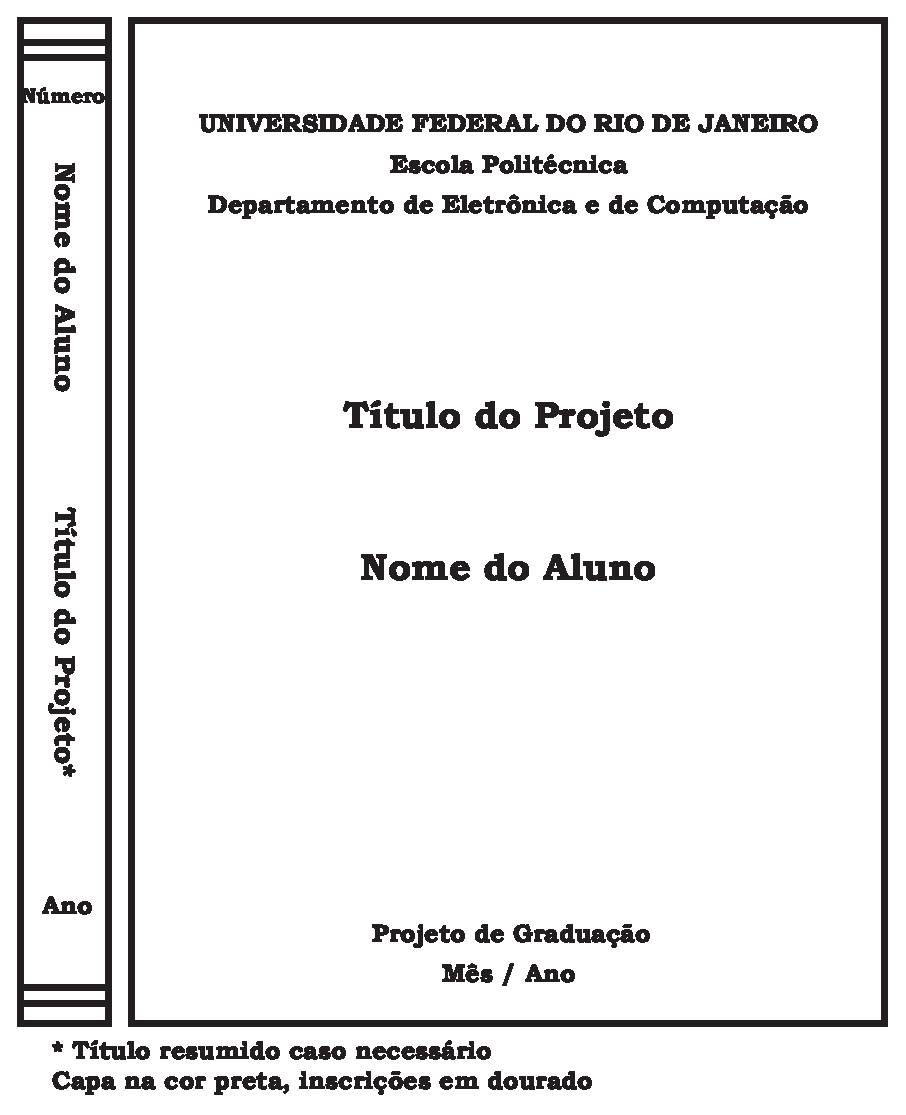
\includegraphics[scale=1.0]{Capa_do_Projeto_Final.eps}
  \caption[\small{Encaderna��o do projeto de gradua��o.}]{\label{FigPFC} \small{Encaderna��o do projeto de gradua��o.}}
  \end{center}
  }
\end{center}
\end{figure}
   % ---------------------------------------------------------------
   % Apêndice C
   % ---------------------------------------------------------------
   \chapter{O que é um anexo}
   \label{ApendiceC}
   \paragraph{}Documentação não elaborada pelo autor, ou elaborada pelo autor mas constituindo parte de outro projeto.   

\backmatter

\end{document}
